The vehicle is modeled using a point mass system driven by a controller providing reference points along the trajectory in latitude ($\lambda$) longitude ($\tau$) coordinates pairs. The equations of motion can be described as 


\begin{align}
\dot{\lambda} &= \frac{1}{(R+h)}V_{g}\cos{\textit{X}_{g}} \\
\dot{\tau} &= \frac{1}{(R+h)\cos{\lambda}}V_{g}\sin{\textit{X}_{g}} \\
\dot{h} &= V_{h}
\end{align}

\vspace{5mm}
where $R$ is Earth's radius, $V_{g}$ is the ground speed, $V_{h}$ is the climb rate, $\textit{X}_{g}$ is the tracking angle, and $h$ is the altitude.

\vspace{10mm}

\begin{figure}
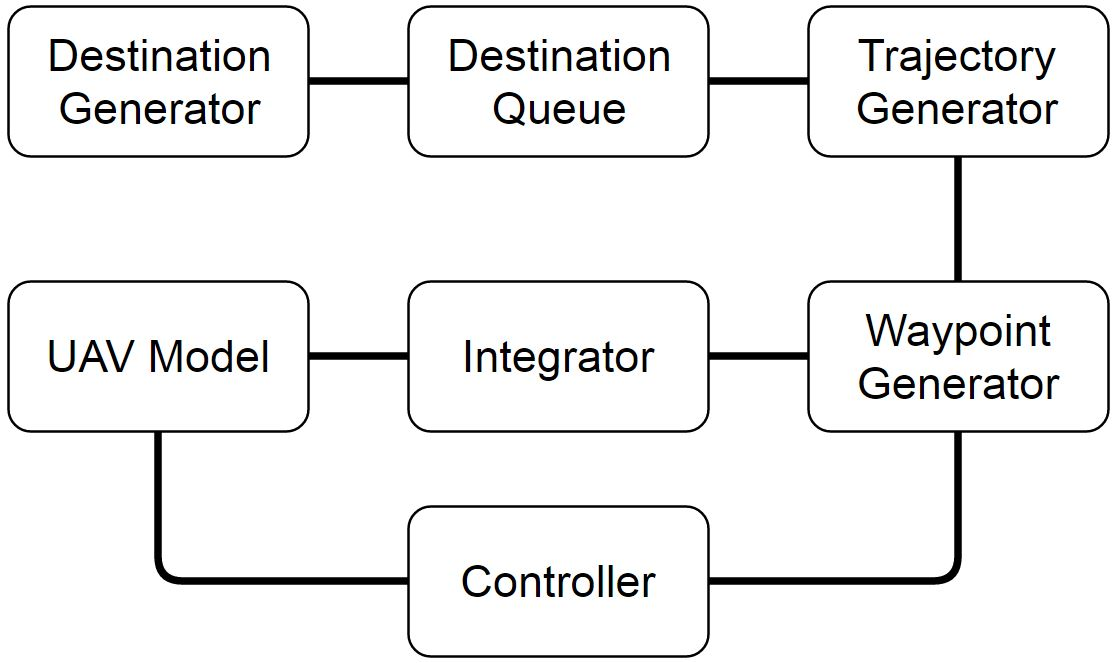
\includegraphics[width=1\linewidth]{images/TopLevelDesign.JPG}
\caption{Simulation Flow Chart}
\end{figure}


